\documentclass[11pt]{article}
\usepackage[margin=1in]{geometry}
\usepackage[T1]{fontenc}
\usepackage{lmodern}
\usepackage{amsmath,amssymb}
\usepackage{booktabs}
\usepackage{graphicx}
\usepackage{xcolor}
\usepackage[numbers,sort&compress]{natbib}
\usepackage[colorlinks=true,linkcolor=blue!50!black,citecolor=blue!50!black,urlcolor=blue!50!black]{hyperref}
\usepackage{caption}
\captionsetup{font=small,labelfont=bf}

\title{Spatially Aware Label-Error Detection\\for Geospatial Machine-Learning Training Data}
\author{Kaisi Omar\\[2pt]
\small London, United Kingdom\\
\small\url{https://github.com/sidewalkds-oss/geolabelqa}}
\date{October 2026}

\begin{document}
\maketitle

\begin{abstract}
Training labels for land-cover and other geospatial models are often wrong, and
the errors are rarely independent. One annotator or one misleading image can
corrupt every label in an area. We study how standard label-error detectors
behave under such spatially clustered errors. On a controlled synthetic
land-cover benchmark (six classes, 3{,}000 samples, five seeds) with uniform,
class-pair and clustered noise, we find three things. First, the common
neighbour-vote check is barely better than chance on clustered errors (average
precision 0.23 at a 20\% error rate where chance is 0.20). Second, confident
learning with random cross-validation is weakened when coordinates are used as
features. Its average precision on clustered errors drops from 0.51 to 0.43, and
spatial block cross-validation recovers it to 0.52, beating random CV in all 15
clustered-noise runs. The price is a small loss when errors are independent.
Third, a simple modification, averaging out-of-fold class probabilities over each
sample's ten nearest spatial neighbours before scoring, improves average precision
in all 180 runs (every noise regime, rate, seed, feature set and CV scheme). The best setting (spectral features, spatial CV,
smoothing) reaches 0.65 on clustered errors. Removing the flagged samples,
however, did not measurably improve a random forest's test accuracy at these noise
levels, and we discuss why. The methods are released as \texttt{geolabelqa}, an
open-source Python package that also validates annotation polygon geometry.
\end{abstract}

%=====================================================================
\section{Introduction}

Supervised land-cover, crop-type and building-extraction models are trained on
labels drawn by people: field surveyors, photo-interpreters and, increasingly,
crowds of annotators working from imagery. Those labels contain errors, and the
cost of the errors is well documented. Label noise lowers the accuracy of the
resulting maps~\citep{pelletier2017effect,mnih2012learning}, and noisy
\emph{evaluation} labels can reorder which model looks best~\citep{northcutt2021pervasive}.
Finding and fixing wrong labels before training is therefore a routine part of
dataset curation.

The standard tools for finding them come from general machine learning. Classifier
filtering~\citep{brodley1999identifying} and confident
learning~\citep{northcutt2021confident} train a model on part of the data,
predict the rest, and flag samples whose given label the model finds unlikely. A
second family of checks is specific to spatial data and older than either. It
appeals to Tobler's first law~\citep{tobler1970computer}: a sample whose label
disagrees with most of its geographic neighbours is suspicious.

Both families assume that errors are \emph{independent}. In geospatial annotation
they often are not. One annotator may consistently confuse cropland with grassland
across their assigned tiles. A cloudy or out-of-date image may mislead every
interpreter who labels a given area. A legacy map used as reference may be wrong
for a whole district. Errors of this kind arrive in \textbf{spatial clusters}, and
both families of checks are blind to them for the same reason. The neighbourhood
check fails because the neighbours share the error. The model-based check fails
whenever the model can learn the local error from nearby training samples. That
happens when coordinates are features, which is common practice, or when features
are themselves spatially autocorrelated. Out-of-fold predictions from
\emph{random} cross-validation then reproduce the mistake instead of contradicting it.

This is the label-auditing counterpart of a problem the mapping community knows
well from model \emph{evaluation}. Random cross-validation on spatially
autocorrelated data gives over-optimistic accuracy estimates, and spatial block
cross-validation is the accepted remedy~\citep{roberts2017cross,valavi2019blockcv,ploton2020spatial,meyer2019importance}.
We argue that the same remedy belongs in label auditing, and that one further step
adds to it: smoothing out-of-fold predictions over geographic neighbours.

\paragraph{Contributions.}
\begin{enumerate}
\item A controlled benchmark that separates three noise regimes (uniform,
  class-pair and spatially clustered) on a synthetic land-cover task with known
  ground truth (Section~\ref{sec:benchmark}).
\item An empirical analysis showing when neighbour voting and random-CV
  confident learning fail, and when spatial block CV restores detection
  (Section~\ref{sec:results}).
\item \emph{Smoothed self-confidence}: a simple, model-agnostic score that
  averages out-of-fold class probabilities over a sample's spatial neighbours
  before ranking (Section~\ref{sec:method}).
\item \texttt{geolabelqa}, an open-source Python package that implements the
  pipeline, together with a dependency-light validator for annotation polygons.
\end{enumerate}

%=====================================================================
\section{Related work}

\paragraph{Label noise.}
\citet{frenay2014survey} survey learning under label noise and distinguish
noise that is completely at random, noise that depends on the class, and noise
that depends on the features. \citet{brodley1999identifying} introduced
classifier filtering, which drops training samples that an ensemble trained on
other folds misclassifies. Confident learning~\citep{northcutt2021confident}
estimates the joint distribution of given and true labels from out-of-fold
probabilities with per-class thresholds. It flags off-diagonal samples and ranks
them by self-confidence, the predicted probability of the given label. These
methods treat samples as exchangeable and say nothing about how to build folds
when samples are spatially dependent.

\paragraph{Label noise in remote sensing.}
\citet{mnih2012learning} trained road and building detectors from misregistered
and incomplete map labels with noise-aware losses. \citet{pelletier2017effect}
measured how random and systematic label noise degrade land-cover classification
from satellite image time series. Systematic noise, where one class is
consistently relabelled as another, hurt more than random noise at the same rate.
Our class-pair and clustered regimes extend that systematic setting by adding
spatial structure.

\paragraph{Spatial cross-validation.}
Spatial autocorrelation violates the independence that random K-fold assumes.
\citet{roberts2017cross} recommend blocking for structured data, and
\texttt{blockCV}~\citep{valavi2019blockcv} made spatial blocking routine in
species-distribution modelling. \citet{ploton2020spatial} showed that
random-CV accuracy for large-scale biomass maps collapsed under spatial
validation. \citet{meyer2019importance} found that coordinates and other
location-proxy predictors encourage models to reproduce training data instead of
generalising. We carry these observations from evaluation over to label auditing.

%=====================================================================
\section{Method}
\label{sec:method}

Let $\{(\mathbf{x}_i, \mathbf{s}_i, \tilde y_i)\}_{i=1}^n$ be training samples
with features $\mathbf{x}_i$, location $\mathbf{s}_i \in \mathbb{R}^2$ in a
projected CRS, and given (possibly wrong) label $\tilde y_i \in \{1,\dots,K\}$.

\paragraph{Out-of-fold probabilities.}
We partition the samples into $F$ folds, train a classifier on $F-1$ folds and
predict class probabilities $\hat{\mathbf{p}}_i \in \Delta^{K-1}$ for the
held-out fold. With \emph{random} CV, folds are a uniform random partition. With
\emph{spatial block} CV, the study area is tiled into square blocks of side $b$,
and whole blocks are assigned to folds. Assignment is greedy, largest block first,
which balances fold sizes. An optional buffer also drops training samples within
distance $r$ of any test sample. When $b$ exceeds the range of spatial
dependence, the model predicting $\hat{\mathbf{p}}_i$ has seen no sample that
shares $i$'s local context, and in particular none that shares a locally clustered
labelling error.

\paragraph{Smoothed self-confidence.}
Let $\mathcal{N}_k(i)$ be the $k$ nearest spatial neighbours of $i$, excluding
$i$. We define the smoothed probability
\begin{equation}
\bar{\mathbf{p}}_i = w\,\hat{\mathbf{p}}_i + (1-w)\,\frac{1}{k}\sum_{j\in\mathcal{N}_k(i)}\hat{\mathbf{p}}_j ,
\end{equation}
and the suspicion score $\sigma_i = 1 - \bar p_{i,\tilde y_i}$. Neighbour
\emph{voting} averages the neighbours' given \emph{labels}, which share any
clustered error. Smoothing averages the neighbours' out-of-fold
\emph{predictions}, which under spatial CV come from models that never saw the
local labels. Smoothing therefore pools independent evidence about the true local
class and lowers the variance of the single-sample prediction. In a spatially
coherent landscape that variance is the main reason correct labels get flagged.
For binary flags we apply the confident-learning rule to $\bar{\mathbf{p}}$:
class $j$ gets threshold $t_j$, the mean of $\bar p_{\cdot j}$ over samples
labelled $j$, and sample $i$ is flagged if the most probable class clearing its
threshold differs from $\tilde y_i$. We use $w = 0.5$ and $k = 10$ throughout and
study both in Section~\ref{sec:ablations}.

\paragraph{Baselines.}
(i) \emph{Neighbour vote}: the share of $\mathcal{N}_{10}(i)$ whose given label
differs from $\tilde y_i$. (ii) \emph{Self-confidence}~\citep{northcutt2021confident}:
$1-\hat p_{i,\tilde y_i}$, which is smoothed self-confidence with $w=1$. Each
model-based score is computed under random and spatial CV.

\paragraph{Geometry validation.}
The class of a polygon label is worth questioning only once its geometry is
sound. \texttt{geolabelqa} also checks GeoJSON annotations against RFC~7946~\citep{rfc7946}
and common topological defects: unclosed rings, too few vertices, repeated
vertices, self-intersection, zero area, slivers (Polsby--Popper compactness
$4\pi A/P^2$ below a threshold~\citep{polsby1991third}), wrong winding order,
holes outside the shell, out-of-range coordinates, duplicate geometries and
missing labels. These checks are not evaluated experimentally here.

%=====================================================================
\section{Benchmark}
\label{sec:benchmark}

\paragraph{Landscape and features.}
A $50\times50$\,km study area is rasterised to $200\times200$ cells. For each of
$K=6$ classes (water, forest, grassland, cropland, urban, bare) we draw white
noise, smooth it with a Gaussian kernel ($\sigma = 6$ cells $= 1.5$\,km) and
standardise it. Each cell takes the class whose field is highest, which yields
irregular homogeneous patches a few kilometres across (Figure~\ref{fig:area}).
We sample $4{,}000$ points uniformly at random: $3{,}000$ for training and
auditing, and $1{,}000$ with clean labels for downstream testing. Each point gets
six surface-reflectance bands (blue to SWIR2) drawn around a class-specific
signature with 30\% relative noise. Grassland and cropland, and urban and bare
soil, have deliberately similar signatures. Reflectance is multiplied by a smooth
illumination field (amplitude 15\%, length scale 3\,km), which mimics atmospheric
and acquisition effects and makes nearby samples similar regardless of class. We
add NDVI, NDWI and NDBI. On clean labels a random forest reaches about 80\%
out-of-fold accuracy, so the task is realistic but not trivial.

\begin{figure}[t]
\centering
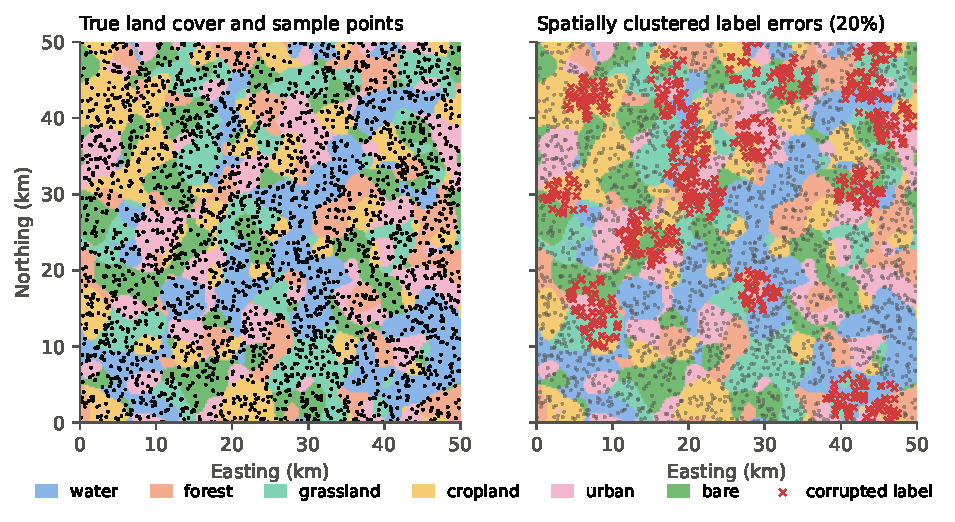
\includegraphics[width=\linewidth]{figures/fig1_study_area.pdf}
\caption{Left: one synthetic landscape with its $3{,}000$ training locations.
Right: the same samples after injecting 20\% spatially clustered label errors.
Each red cross is a sample whose label was changed to its class's look-alike.}
\label{fig:area}
\end{figure}

\paragraph{Noise regimes.}
Each class has a look-alike class (water$\to$forest, forest$\to$grassland,
grassland$\leftrightarrow$cropland, urban$\leftrightarrow$bare). At rate
$\rho\in\{0.1,0.2,0.3\}$ we corrupt exactly $\rho n$ labels:
\begin{itemize}
\item \textbf{Uniform}: random samples are relabelled to a uniformly random other class.
\item \textbf{Class-pair}: random samples are relabelled to their look-alike class.
\item \textbf{Clustered}: discs of radius 3\,km centred on random samples are
  added until $\rho n$ samples are covered, and every sample inside is relabelled
  to its look-alike. This models a regionally systematic annotator or imagery error.
\end{itemize}

\paragraph{Protocol.}
The classifier is a random forest~\citep{breiman2001random} (100 trees, minimum
leaf size 2) from scikit-learn~\citep{pedregosa2011scikit}, with $F=5$ folds.
Spatial CV uses $b=10$\,km blocks (25 blocks). We compare two feature sets:
\emph{spectral} (9 features) and \emph{spectral\,+\,x,y}, which appends the
coordinates as many geospatial ML pipelines do. Every configuration is repeated
with 5 seeds; each seed redraws the landscape, the samples and the noise. We report
average precision (AP) for ranking corrupted samples (chance equals $\rho$), and
precision, recall and F1 of the confident-learning flags. For downstream impact we
remove the $\rho n$ highest-scoring samples (the true error count, so every method
gets the same review budget), retrain, and report macro-F1 on the clean test set.

%=====================================================================
\section{Results}
\label{sec:results}

Table~\ref{tab:detection} reports average precision at a 20\% error rate for
every combination of detector, feature set and CV scheme. Figure~\ref{fig:rates}
shows the trend across error rates for the spectral\,+\,x,y setting.

\begin{table}[t]
\centering\small
\caption{Average precision for ranking corrupted labels at a 20\% error rate
(mean $\pm$ s.d.\ over 5 seeds; chance $=0.20$). Bold marks the best entry per column.}
\label{tab:detection}
\resizebox{\linewidth}{!}{\begin{tabular}{lll ccc}
\toprule
Detector & Features & CV & Uniform & Class-pair & Clustered \\
\midrule
Neighbour vote & -- & -- & 0.813 $\pm$ 0.014 & 0.613 $\pm$ 0.003 & 0.234 $\pm$ 0.021 \\
Self-confidence & spectral & random & 0.908 $\pm$ 0.011 & 0.535 $\pm$ 0.008 & 0.513 $\pm$ 0.038 \\
Self-confidence & spectral & spatial & 0.902 $\pm$ 0.014 & 0.519 $\pm$ 0.021 & 0.543 $\pm$ 0.061 \\
Smoothed SC (ours) & spectral & random & 0.944 $\pm$ 0.011 & 0.630 $\pm$ 0.023 & 0.614 $\pm$ 0.053 \\
Smoothed SC (ours) & spectral & spatial & 0.939 $\pm$ 0.009 & 0.610 $\pm$ 0.023 & \textbf{0.653 $\pm$ 0.072} \\
Self-confidence & spectral + x,y & random & 0.931 $\pm$ 0.009 & 0.579 $\pm$ 0.019 & 0.427 $\pm$ 0.045 \\
Self-confidence & spectral + x,y & spatial & 0.910 $\pm$ 0.013 & 0.523 $\pm$ 0.019 & 0.519 $\pm$ 0.061 \\
Smoothed SC (ours) & spectral + x,y & random & \textbf{0.957 $\pm$ 0.008} & \textbf{0.672 $\pm$ 0.033} & 0.478 $\pm$ 0.063 \\
Smoothed SC (ours) & spectral + x,y & spatial & 0.940 $\pm$ 0.007 & 0.607 $\pm$ 0.025 & 0.588 $\pm$ 0.067 \\
\bottomrule
\end{tabular}}
\end{table}

\begin{figure}[t]
\centering
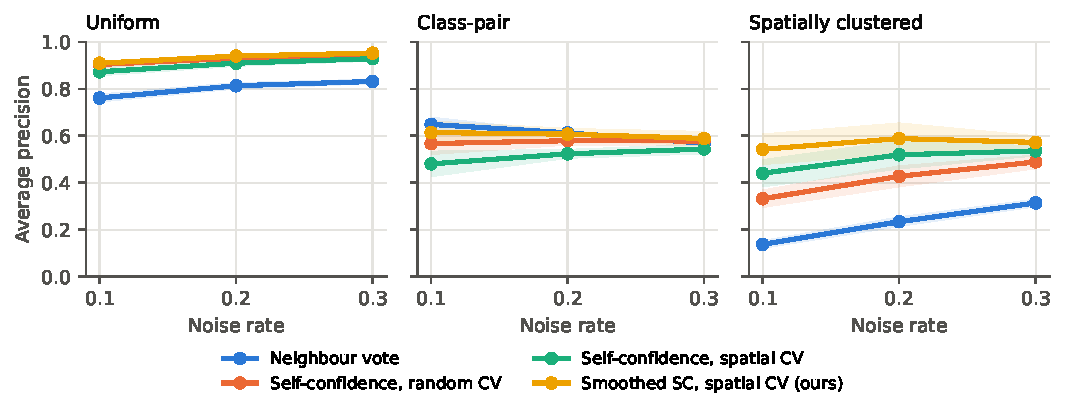
\includegraphics[width=\linewidth]{figures/fig2_ap_vs_rate_xy.pdf}
\caption{Average precision versus error rate, features = spectral\,+\,x,y.
Bands show $\pm1$ s.d.\ over 5 seeds. Clustered errors separate the methods;
independent errors do not.}
\label{fig:rates}
\end{figure}

\paragraph{Neighbour voting fails on clustered errors.}
With uniform errors, neighbour voting is a reasonable detector (AP 0.81). It is
also the strongest raw score for class-pair errors at low rates (0.65 at 10\%),
because an isolated look-alike label stands out in a homogeneous patch. With
clustered errors it collapses to AP 0.23 and AUROC 0.57, barely above chance.
This is the expected failure, and it is total: a clustered error is
surrounded by samples carrying the same error.

\paragraph{Coordinates plus random CV hide clustered errors.}
Self-confidence with random CV reaches AP 0.51 on clustered errors using spectral
features alone. Adding coordinates as features lowers it to 0.43, and to 0.33 at
a 10\% error rate. The forest learns where the mislabelled patches are and
predicts the wrong label back. Spatial block CV removes that shortcut and restores
AP to 0.52. With coordinates as features, spatial CV beat random CV in 15 of 15
clustered-noise runs (5 seeds $\times$ 3 rates). For spectral features alone the
gain is smaller (0.51$\to$0.54), consistent with the weaker spatial signal that
the smooth illumination field carries.

\paragraph{Spatial CV has a cost under independent errors.}
The same comparison reverses when errors are independent. Random CV beat spatial
CV in all 30 uniform and class-pair runs with coordinates, by 0.02 AP (uniform)
and 0.06 AP (class-pair) at 20\%. With random folds the model sees training
samples from the same patch. That helps when those neighbours are correctly
labelled, which is the case under independent noise. Spatial CV is therefore
insurance: a small premium when errors are independent, a large payout when they
are clustered. Because the error process is unknown in practice, we consider the
premium worth paying.

\paragraph{Smoothing helps everywhere.}
Smoothed self-confidence improved AP over raw self-confidence in all 180 runs
(3 regimes $\times$ 3 rates $\times$ 5 seeds $\times$ 2 feature sets $\times$ 2 CV
schemes). With coordinates and spatial CV, the gains at 20\% were $+0.03$
(uniform), $+0.08$ (class-pair) and $+0.07$ (clustered). With coordinates and
random CV the clustered-noise gain was smaller ($+0.05$), because the
neighbours' predictions share the leaked error. The best clustered-noise result overall is
smoothed self-confidence with spectral features and spatial CV (AP 0.65,
precision 0.61 at the true error count).

\paragraph{Confident-learning flags.}
Table~\ref{tab:clflags} applies the confident-learning flag rule to raw and
smoothed probabilities (spectral\,+\,x,y, spatial CV). Smoothing raises precision
in every regime, for example 0.54$\to$0.61 on uniform errors, at a small cost in
recall, and F1 rises slightly. The flags recover about half of clustered errors at
0.45 precision, so a human reviewer should treat them as a work queue, not as
automatic corrections.

\begin{table}[t]
\centering\small
\caption{Confident-learning flags: precision / recall / F1 at a 20\% error rate
(spectral\,+\,x,y, spatial CV, mean over 5 seeds).}
\label{tab:clflags}
\begin{tabular}{l ccc}
\toprule
Confident-learning flags on & Uniform & Class-pair & Clustered \\
\midrule
Raw probabilities & 0.54 / 0.82 / 0.65 & 0.46 / 0.62 / 0.53 & 0.41 / 0.54 / 0.46 \\
Smoothed probabilities (ours) & 0.61 / 0.80 / 0.69 & 0.54 / 0.60 / 0.57 & 0.45 / 0.50 / 0.47 \\
\bottomrule
\end{tabular}
\end{table}

\paragraph{Downstream accuracy.}
Table~\ref{tab:downstream} reports test macro-F1 after removing the $\rho n$
most suspicious samples. The results are a negative finding. The random forest
is robust to 20\% uniform or class-pair noise (0.805 and 0.789 against 0.812 with
clean labels), so there is little to recover. For clustered noise there is a real
gap (0.759 against 0.810 when every corrupted sample is removed), but no detector
closes it. Smoothed self-confidence gains only 0.004, and neighbour voting makes
matters worse. At AP $\approx 0.6$, removing the top-$n$ discards many correct
samples near the corrupted patches as well as the corrupted ones. The rest of each
corrupted patch is left in place, and it still teaches the error. Better
detection rankings do not by themselves translate into better models. Relabelling
flagged samples, rather than removing them, and auditing iteratively are natural
next steps.

\begin{table}[t]
\centering\small
\caption{Test macro-F1 on clean labels after removing the top-$n$ suspicious
training samples ($n$ = true error count), 20\% error rate, spectral\,+\,x,y
features (mean $\pm$ s.d.\ over 5 seeds).}
\label{tab:downstream}
\resizebox{\linewidth}{!}{\begin{tabular}{l ccc}
\toprule
Training labels & Uniform & Class-pair & Clustered \\
\midrule
No cleaning & 0.805 $\pm$ 0.025 & 0.789 $\pm$ 0.022 & 0.759 $\pm$ 0.027 \\
\midrule
Remove top-$n$: neighbour vote & 0.815 $\pm$ 0.020 & 0.807 $\pm$ 0.024 & 0.740 $\pm$ 0.027 \\
Remove top-$n$: SC, random CV & 0.807 $\pm$ 0.016 & 0.781 $\pm$ 0.011 & 0.758 $\pm$ 0.015 \\
Remove top-$n$: SC, spatial CV & 0.798 $\pm$ 0.020 & 0.778 $\pm$ 0.012 & 0.759 $\pm$ 0.013 \\
Remove top-$n$: smoothed SC, spatial CV (ours) & 0.804 $\pm$ 0.018 & 0.779 $\pm$ 0.016 & 0.763 $\pm$ 0.013 \\
\midrule
Oracle: remove all corrupted & 0.810 $\pm$ 0.019 & 0.810 $\pm$ 0.019 & 0.810 $\pm$ 0.020 \\
Oracle: all labels correct & 0.812 $\pm$ 0.015 & 0.812 $\pm$ 0.015 & 0.812 $\pm$ 0.015 \\
\bottomrule
\end{tabular}}
\end{table}

%=====================================================================
\section{Ablations}
\label{sec:ablations}

\paragraph{Smoothing strength.}
Figure~\ref{fig:smoothing} varies the self-weight $w$ and neighbourhood size $k$.
Every regime peaks at $w=0.5$, and small neighbourhoods ($k=5$ or $10$) are best.
At $w=0$ the sample's own prediction is discarded and AP falls well below the
unsmoothed score. The method is therefore a variance-reduction step around the
sample's own prediction, not a replacement for it. With $k=40$ the neighbourhood
spans patch boundaries and the gain shrinks. A natural default is $k$ set so that
neighbourhoods stay within typical patch sizes.

\begin{figure}[t]
\centering
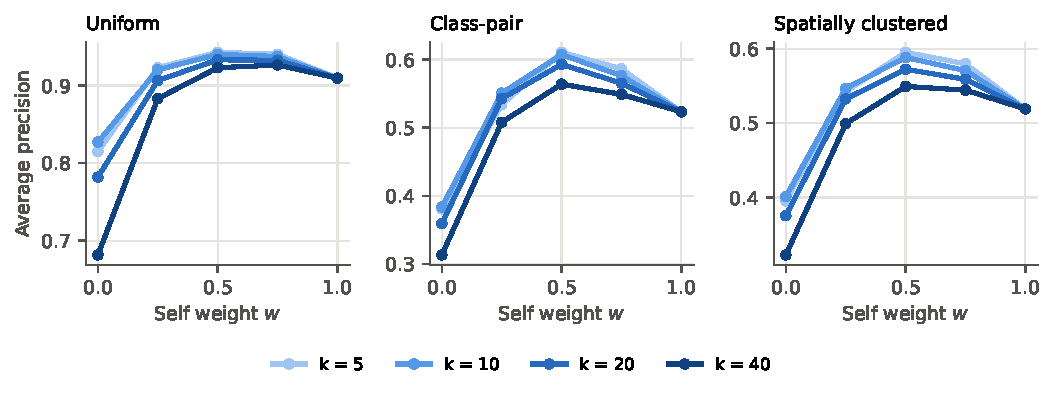
\includegraphics[width=\linewidth]{figures/fig3_smoothing_ablation.pdf}
\caption{AP of smoothed self-confidence versus self-weight $w$ ($w=1$: no
smoothing) and neighbourhood size $k$. 20\% error rate, spectral\,+\,x,y,
spatial CV, mean over 5 seeds.}
\label{fig:smoothing}
\end{figure}

\paragraph{Block size.}
Table~\ref{tab:block} varies the spatial CV block size for clustered noise. Blocks
of 2.5 or 5\,km are similar in size to the 3\,km-radius error discs and leave the
shortcut partly open. 10\,km blocks are best. 20\,km blocks (only three columns
of blocks across the area, for five folds) start to starve the model of training
diversity. This mirrors the guidance from spatial model evaluation: blocks should
exceed the range of dependence, here the size of the error clusters, but not by
so much that folds stop being representative~\citep{roberts2017cross,valavi2019blockcv}.

\begin{table}[t]
\centering\small
\caption{Effect of block size on clustered-error detection (AP, 20\% error rate,
spectral\,+\,x,y, mean $\pm$ s.d.\ over 5 seeds).}
\label{tab:block}
\begin{tabular}{c cc}
\toprule
Block size (km) & Self-confidence & Smoothed SC \\
\midrule
2.5 & 0.456 $\pm$ 0.034 & 0.513 $\pm$ 0.052 \\
5 & 0.472 $\pm$ 0.054 & 0.529 $\pm$ 0.063 \\
10 & 0.519 $\pm$ 0.061 & 0.588 $\pm$ 0.067 \\
20 & 0.497 $\pm$ 0.039 & 0.569 $\pm$ 0.064 \\
\bottomrule
\end{tabular}
\end{table}

%=====================================================================
\section{Discussion and limitations}

\paragraph{Practical recommendations.}
(1) Do not rely on neighbour voting alone: it cannot see the errors that matter
most in geospatial annotation. (2) Audit with spatial block CV, even though it is
slightly worse when errors happen to be independent. (3) Keep coordinates and
other location proxies out of the auditing model, even if the production model
uses them~\citep{meyer2019importance}. (4) Smooth out-of-fold probabilities over a
small spatial neighbourhood ($k\approx10$, $w=0.5$) before ranking. (5) Use the
ranking to direct human review; at the precision reached here, automatic removal
did not pay off.

\paragraph{Limitations.}
All results come from a synthetic benchmark. Its value is that the error process
is known exactly, which real data rarely allows. But the landscape model, the
spectral signatures and the disc-shaped error clusters are simplifications. Real
annotation errors may follow tile boundaries, image dates or class-specific
difficulty. We used one classifier family (random forest) and one sample size, and
did not tune block size or $k$ per dataset beyond the ablations shown. The next
step is validation on public land-cover reference datasets with documented or
re-verified label errors. A second is combining smoothing with confident
learning's full noise-matrix estimation, rather than its ranking alone.

%=====================================================================
\section{Conclusion}

Spatially clustered label errors defeat the two most common audit checks for
geospatial training data: neighbour voting and confident learning with random
folds. Spatial block cross-validation restores model-based detection, and
smoothing out-of-fold probabilities over spatial neighbours improves it further
at no extra training cost. Both are implemented in \texttt{geolabelqa}, which also
checks annotation geometry, and the full benchmark can be reproduced with two
commands.

\paragraph{Reproducibility.}
\texttt{python experiments/run\_benchmark.py} regenerates every CSV in
\texttt{results/} (about 30 minutes on a laptop CPU), and
\texttt{python experiments/make\_figures.py} regenerates every figure and table
in this paper.

\bibliographystyle{plainnat}
\bibliography{references}

\end{document}
